\chapter{Designs and Performance Modeling}

Two CNN models - GoogLeNet (inception V1) and Resnet-50 - were implemented on FPGAs in the project. The choices were made based on :  
\begin{itemize}
  \item complexity of CNN models
  \item relevance in the industry
  \item accuracy of the models
  \item availability of pre-trained weights and biases
  \item project timeline
\end{itemize}  
We wanted to implement CNN models complex enough to require scaling over multiple FPGAs. This requirement was a direct consequence of our initial objective of wanting to scale over multiple FPGA devices. Here, the complexity of the model refers the number of hidden layers present in the model. GoogLeNet - with  xyz\todo{Add layer count} layers - and Resnet - with abc \todo{Add layer count} layers- are deep enough to warrant using multiple devices for implementing them.

As the winners of Imagenet Large Scale Visual Recognition Challenge(ILSVR) 2014 and 2015 respectively, GoogLeNet and Reset are quite well known in the industry. With an inference accuracy nearing human capability - GoogLeNet or exceeding human capability -Resnet-152, these models are very popular in the machine learning community. 

Since our objective was to implement an inference engine and not training an inference engine , it was imperative to work with models for which weights and biases were readily available. The popularity of GoogLeNet and Resnet in the machine learning community meant that the weights and biases were available freely in the form of frozen models \todo{Explain frozen models?}.

We stopped at two models as the time required to implement more models was significant and would have forced us to spend less time on other important tasks. And the main objective of our project - implementing CNNs on FPGAs - was met when we successfully implemented GoogLeNet and Resnet. We felt no additional findings would come out of implementing another CNN model on FPGAs.

Implementation of such complex applications on FPGAs calls for "Performance Modeling". Performance Modeling entails the detailed study of how kernels get executed on FPGAs. Performance Modeling allows a design engineer to understand the bottlenecks, performance limiting issues, general performance etc of kernels. Using performance modeling and making an educated assumption about the final design clock frequency, a design engineer can also predict the approximate run-time of a design.
For all the designs which we implemented, we also created models to explain the performance of our designs.    

In the next few sections, we explain in detail how we implemented different FPGA designs of GoogLeNet and Resnet-50 and the accompanying performance models.



\section{GoogLeNet}

The first CNN model we implemented was GoogLeNet. The idea of multiple designs of GoogLeNet was hatched to see the difference in performances when different levels of optimizations are applied at OpenCL level and architectural level. 
We were able to implement three major designs for GoogLeNet :
\begin{itemize}
  \item Baseline
  \item DSP Usage Optimized
  \item Hybrid Design
\end{itemize}  

\subsection{GoogLeNet Baseline}

GoogLeNet Baseline was implemented by modifying the OpenCL code generated by TVM for GoogLeNet. We modified the generated code to meet the requirements of our plugin. Some of the major modifications which were performed are :
\begin{itemize}
  \item renaming kernel names
  \item merging ReLUs with Convolutions
  \item rewriting Concatenation layers to support NCHW layout
  \item removing transpose kernels
\end{itemize}  
We had to rename kernels as the naming convention used by TVM and our plugin was not the same. We  had to make sure that we had all the kernels in OpenCL code that the plugin expected to launch.

By merging ReLUs with Convolutions, we optimized away the need to send data from one kernel(Convolutions) to another(ReLUs). This preoptimization step is used in the Deep Learning Community widely as ReLUs are basically light weight operations and do not warrant separate kernels.

By analysing our plugin, which is an extension to OpenVINO, and TVM, we realized that the layout used by OpenVINO and TVM were quite different. OpenVINO uses NCHW layout scheme whereas TVM uses NHWC layout scheme in Concatenation layer and NCHW layout scheme in all the other layers. To convert from NHWC to NCHW, TVM had generated transpose kernels. We modified all the Concatenation kernels to output NCHW thereby eliminating the need to have transpose layers.  

The modified code was first compiled to run on an FPGA emulator \todo{Insert correct name for emulator}. We verified the functional correctness of the modified code by comparing the values output by our modified code with the values output by TensorFlow implementation of the same model.  

The initial reports generated for this modified OpenCL code indicated that this implementation of GoogLeNet was far too big to fit on a single Stratix 10 board. In order to successfully run this design on FPGAs, there was a need to divide the design into smaller parts. By dividing the design into ten smaller parts, we took advantage of the inherent logical divisions present in GoogLeNet topology. As  described in \ref{GoogLeNet_Topo}, every inception module is followed by a  Concatenation layer. Thus, we divided our design into ten smaller parts.  The first part is a purely feed forward design. The rest of the parts contain at least one inception module each and other layers as shown in Figure \ref{fig:GoogLeNet_division}


\begin{figure}[h!]
  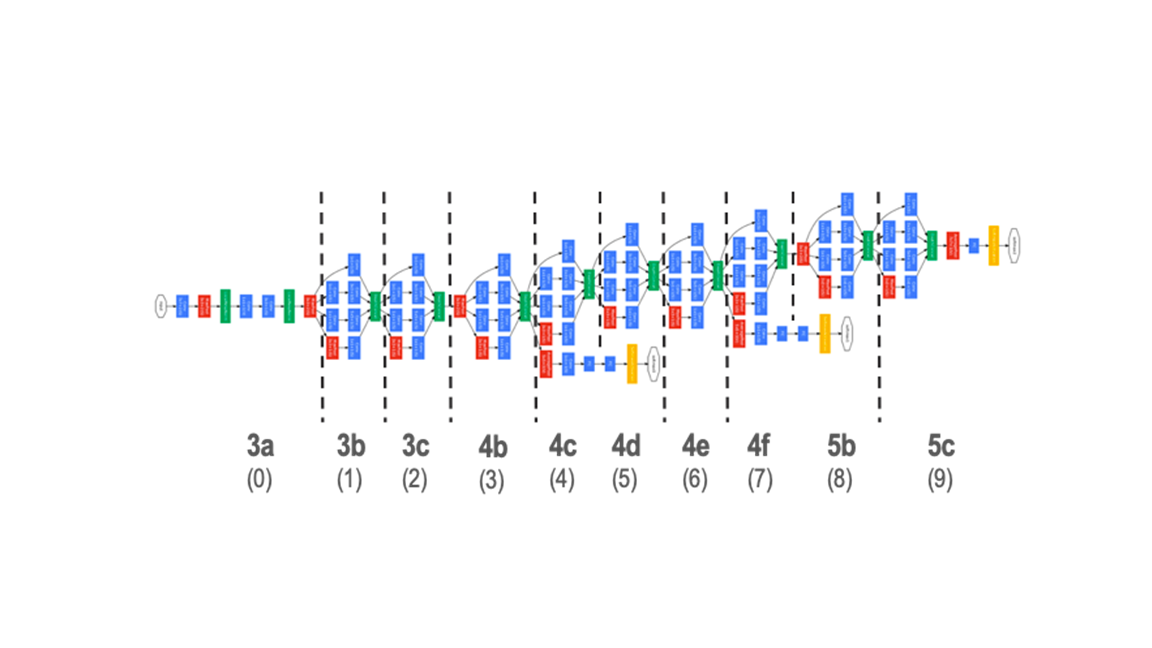
\includegraphics[width=\textwidth,height=\textheight,keepaspectratio]{img/GoogLeNet_division.png}
  \caption{Division of GoogLeNet topology}
  \label{fig:GoogLeNet_division}
\end{figure}
 
The ten resulting OpenCL bitstream files (in aocx format) were named as "inceptionX", where X represents the ordinal value(shown in brackets) of the part the file is made of as shown in Figure \ref{fig:GoogLeNet_division}. For example, the file containing the description of part 3a in Figure \ref{fig:GoogLeNet_division} was named as "inception0.aocx". This naming convention plays a crucial part in deciding the order in which the bitstreams are flashed on multiple devices as discussed further ahead in this section.  

We envisioned scaling over ten devices by using the scheme shown in Figure \ref{fig:GoogLeNet_Scaling}

\begin{figure}[h!]
  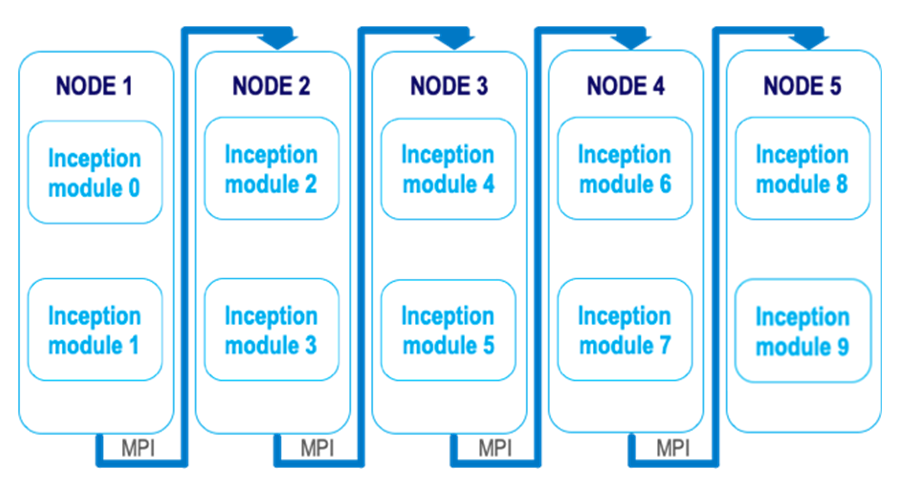
\includegraphics[width=\textwidth,height=\textheight,keepaspectratio]{img/GoogLeNet_Scaling.png}
  \caption{Scaling of GoogLeNet topology over 10 FPGAs}
  \label{fig:GoogLeNet_Scaling}
\end{figure}

Each Noctua FPGA node has two FPGAs. Thus, this scheme requires five nodes to execute ten parts of GoogLeNet. Right off the bat, we had two main challenges - flashing the right bitstreams on to the right devices, and transferring data from one node to another.

The first challenge - flashing the right bitstreams on to the right devices was solved using Message Passing Interface (MPI). This is shown in Listing \ref{code:MPICode_plugin}.  


\begin{code}[!htb]
 \begin{minted}{c++}
 /* Snippet of test plugin - main.cpp */
        #include "mpi.h"
        MPI_Init(NULL,NULL);
        int rank;
        MPI_Comm_rank(MPI_COMM_WORLD,&rank);
        fpga_launcher(network,inputModel,imageNames,cnn_model,rank);
    
\end{minted}
\captionof{listing}{testplugin/main.cpp}
\label{code:MPICode_plugin}
\end{code}

We included the MPI library and initialized it. We retreived the rank of the nodes and then passed the ranks as parameter to the function \texttt{"fpga\_launcher()"}. This function is present in \texttt{"noctua\_plugin /fpga\_plugin.cpp"}. With the ranks as parameters , this function handles the flashing of the bitstreams by calculating the parity of the ranks. These ranks in themselves are enough to identify the nodes(since the ranks are retrieved from the nodes). This is shown in Listing \ref{code:MPICode_fpga_plugin}.

\begin{code}[!htb]
 \begin{minted}{c++}
 /* Snippet of noctua_plugin - fpga_plugin.cpp */
        #include "mpi.h"  
        
        std::string file1 = GoogLeNet_DIR+"inception"+std::to_string(2*rank)+".aocx" 
        std::string file2 = GoogLeNet_DIR+"inception"+std::to_string(2*rank+1)+".aocx"  
        
        std::string file1_xml = GoogLeNet_DIR+"inception"+std::to_string(2*rank)+".xml"
        std::string file2_xml = GoogLeNet_DIR+"inception"+std::to_string(2*rank+1)+".xml"   
        
        char f1_xml[file1_xml.length()];
        strcpy(f1_xml,file1_xml.c_str());  
        
        std::vector<std::string> first_kernels = xml_parser1(f1_xml);

\end{minted}
\captionof{listing}{noctua\_plugin/fpga\_plugin.cpp}
\label{code:MPICode_fpga_plugin}
\end{code}

The naming convention we used for the bitstreams allowed us to pick the appropriate bitstreams by  name and thus, we successfully flashed the bitstreams on to the correct devices. We also read and parsed the XML files which were generated along with the bitstreams. These XML files contain information about the kernels present in a particular bitstream. Using this information, we launched all the valid kernels as needed. 

The second challenge - transferring data from one node to another was also solved using MPI. The devices in a node share the same memory address space and thus , they had access to each other`s global memory.   

The data transfers from one device to another device in the same node were handled using global memory. The data transfers from a device on one node to a deivce on another node was handled using two MPI functions : MPI\_Send() and MPI\_Recv(). We called MPI\_Send() at the last kernel of every node except for the very last one. And the first kernel of every node had a function call for MPI\_Recv(). The visual representation of this scheme is show in Figure \ref{fig:GoogLeNet_Scaling}. Thus, using  MPI\_Send() and MPI\_Recv(), we were able to transfer data from one node to another, allowing us to truly scale over multiple devices.

This implementation of GoogLeNet is completely devoid of optimizations barring a few implementation related optimizations (merging ReLUs with Convolutions etc). Thus, it was named as "Baseline". When we executed this baseline version of GoogLeNet over ten devices, the design took 67.47 seconds to classify one image.  

By any measure, this execution time is extremely slow when it comes to designs running on accelerators. To see why this baseline was slow , we had to first do performance modelling to explain this run time.

The performance modeling for designs like this involves determining
  Multiply-Accumulate (MAC) operations in design , amount of global memory transfers, run-time, clock frequency ,and the initiation intervals (IIs) and latency of loops.

The run-time and clock frequency are ascertained from "profile.mon" files.   
The profiling data generated by Intel SDK for OpenCL Applications are stored in files named "profile.mon". These are generated whenever kernels are executed on FPGAs. During synthesis, it is necessary to enable -profile flag if one wishes to have profiling data generated for their designs (when they are executed on FPGAs). We had enabled this flag for all our designs and thus had access to profiling data for all our kernels.

The first two steps of performance modeling for baseline - determining number of operations and amount of global memory transfers - were done using a script developed by the team. The script was written in Python and made use of ANTLR4 lexer and parser generator tool. OpenCL follows the grammar of C language. Keeping this in mind, we generated a parse tree of all the ten OpenCL source files with the help of ANTLR4 using C.g4 grammar file (Grammar files use the "g4" file extension). We wrote a script to walk the parse tree to determine the number of MAC operations and the amount of global memory transfers present in a file.

The next two steps of performance modeling - determining execution time and clock frequency - were done by opening profile.mon files using the profie.mon viewer provided by Intel SDK for OpenCL. The profiling data records execution time of each and every single kernel which get executed to completion. And the overall frequency at which the kernels in a given OpenCL file run is also recorded in these files.The initiation intervals and latency of different parts of loops is gathered from HTML reports. Taking all this into consideration , the performance modeling of baseline design revealed the details tabulated in Table \ref{tab:GoogLeNetBaselinePerfModel} 
\begin{table}[!htb]                          
 \centering
    \begin{tabular}{|c|c|}
    \multicolumn{2}{c}{\textbf{GoogLeNet Baseline : Performance Model}} \\ \hline

     No.of Operations    &   2.9 Billion \\ \hline
      Global Mem transfers &   20.9 GB            \\ \hline          
      Exe time    &  67470 ms    \\ \hline
      Operations/second   &   0.04 GOPS \\ \hline
      Operations/cycle &   0.216             \\ \hline
      Operations/byte       &   0.143     \\ \hline
      Global mem/second & 311 MBps  \\ \hline

    \end{tabular}
    \caption{GoogLeNet Baseline Performance Model}
    \label{tab:GoogLeNetBaselinePerfModel}                            

\end{table}  

Throughput, as defined in Chapter \ref{chp:Metrics}, for this design is 0.014 images classified per second. Since accuracy of the model is same as the one given in the literature (93.33\%), the only factor that could change when calculating Rate Correct Score is the latency. And for this case , Rate Correct Score is calculated as the ratio between accuracy from literature and the latency of our implementation of GoogLeNet. This comes to be  1.38/second.

The HTML reports revealed that the initiation intervals of most of the loops were much bigger than 1. And some of the loops were not pipelined.There were loop-carried dependencies as well. We also observed from initial reports that the DSP usage of Baseline was quite abysmal. Baseline design was using only about 1\% of the total DSPs available on Stratix 10 board. This is shown in Figure \ref{fig:Report_Baseline}   


\begin{figure}[!htb]
  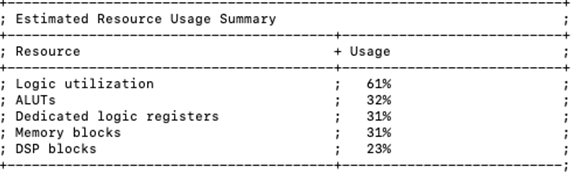
\includegraphics[width=\textwidth,height=\textheight,keepaspectratio]{img/Report_Baseline.png}
  \caption{Initial report of one of the files of Baseline Design}
  \label{fig:Report_Baseline}
\end{figure}

Though the estimated DSP blocks usage is 23\% in Figure \ref{fig:Report_Baseline} , in reality only 1\% of the DSP blocks is used by the design as the overhead required by the board takes up about 22\% of the DSP blocks. The rest remain untouched,unused by our design.

Furthermore, the profiling data for baseline also indicated that the occupancy of  parts of the code where the MAC operations take place were extremely low - in the neighbourhood of 0.1\%. 

Since none of the loops were unrolled, and because of loop carried dependencies (compiler would not unroll automatically), we could estimate that only two operations would take place in one cycle (the inner most loop has two operations - one multiply and one addition). If the loops were unrolled , then the design could have utilized more number of DSP blocks in a single clock cycle thereby executing more number of operations per cycle. In reality (from measurements), we saw that the real operations/cycle was 0.216 (as opposed to an estimated 2 ops/cycle). This indicated that even the resources (DSP blocks specifically) which were assigned were underused.Additionally, the low utilization of DSP blocks indicates the biggest problem with this design - lack of parallel execution of operations.  

As shown in Figure \ref{fig:GoogLeNetBaseline_Runtime_Graph} , we notice that the slowest kernel was at the top of the design - a 3x3 convolution kernel. It took about 18s to get executed. "Inception0" has the most number of operations in the design and it is not surprising that it took the lion`s share of the total time to get executed to completion. Every other 3x3 convolution kernel also took significant amounts of time to get executed. Other kernels - like padding and concatenation kernels were relatively fast. The graph in Figure \ref{fig:GoogLeNetBaseline_Runtime_Graph} helps us visualize the execution sequence of the design. Once execution on the first FPGA is over, the execution takes place in the second one. And once the image is processed in the second FPGA, it moves on to the thrid FPGA and so on. Most of the times the FPGAs remain idle as can be seen from the empty regions in the time axis in the graph. The total execution time, as mentioned above, was 67.47 seconds.

\begin{figure}[!htb]
  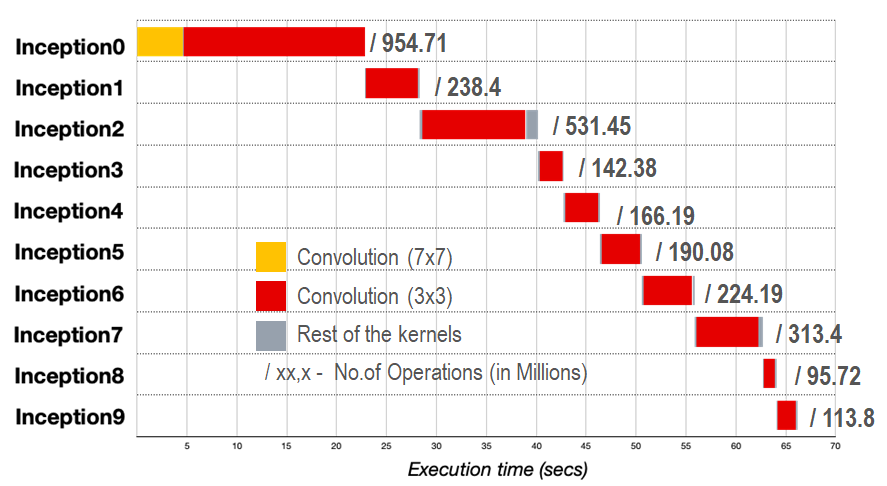
\includegraphics[width=\textwidth,height=\textheight,keepaspectratio]{img/GoogLeNetBaseline_Runtime_Graph.png}
  \caption{Execution time - GoogLeNet Baseline Design}
  \label{fig:GoogLeNetBaseline_Runtime_Graph}
\end{figure}

In conclusion, the reasons for baseline version of GoogLeNet performing so badly are :
\begin{itemize}
    \item low DSP blocks usage
    \item initiation intervals greater than 1
    \item loop carried dependencies 
    \item global memory transfers
    \item FPGAs remain idle most of the time
\end{itemize}

To speed this design up, we decided to solve the problem of low DSP usage. This leads us to our next section - GoogLeNet DSP Usage Optimized.

\subsection{GoogLeNet DSP Usage Optimized}
The biggest problem with the baseline implementation of GoogLeNet, according to us, was the very low utilization of DSP blocks (or just DSPs). With an estimated two operations per one clock cycle, it is easy to see that such a design is doomed to have very bad performance (given the clock frequencies are in hundreds of MHz range).
 
Keeping this in mind, we decided to increase the number of operations our design could perform in one clock cycle. As was noted in the previous section, an increase in number of DSPs could result in more number of operations getting executed in one clock cycle. If the inner most loops are unrolled, then the compiler allocates an increased number of resources to carry out all these unrolled operations in parallel (given that these operations have an II of 1 - no dependencies between operations). 
 
 Thus, in order to have an increased allocation of DSPs to our design, we made use of interrelated  optimization techniques like : 
 \begin{itemize}
     \item Loop Unrolling
     \item Loop Pipelining
     \item Using Shift Registers
     \item Using Local Memory
\end{itemize}

When these optimization techniques were applied on the baseline design, we were able to increase the total DSPs by a margin of just 1\%. Which was quite disappointing. The problem lay in the fact that we were limited by the amount of unrolls we could perform. After unrolling by a few factors, we noticed that the other resources` usage would go beyond what was available on Stratix 10 boards.  

This problem was intrinsic to the convolution logic the design had. We observed that the operations were happening depth wise first and then along the spatial dimension. This convolution logic is depicted in Figure \ref{fig:GoogLeNet_Conv_logic}.This logic works by first operating on pixels along the red arrow first (depth wise). Then it moves to the next pixel in the spatial dimension and continues working with the pixels depth wise 

\begin{figure}[!htb]
  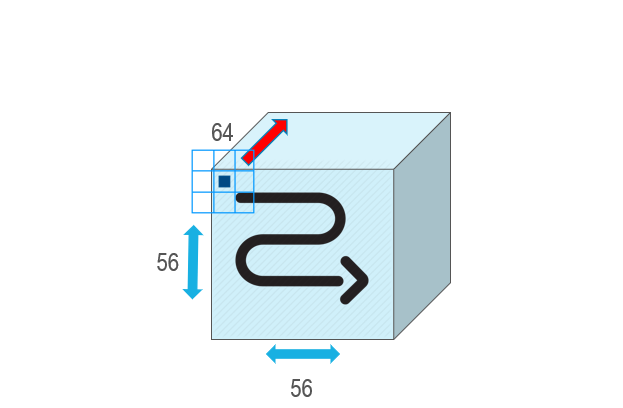
\includegraphics[width=\textwidth,height=\textheight,keepaspectratio]{img/GoogLeNet_Conv_logic.png}
  \caption{Example of Convolution Logic}
  \label{fig:GoogLeNet_Conv_logic}
\end{figure}

Unrolling the loops which work with the above logic results in replicating the big image-data (as shown in Figure \ref{fig:GoogLeNet_Conv_logic}, dimensions vary from kernel to kernel) multiple times. After just a few unrolls, we start to reach the limits of resources available Stratix 10 board. Thus, the idea of simply unrolling the inner most loop just would not work with the logic present in this design,

To overcome this problem, we decided to change the order of the loops such that the calculations happen on the spatial plane first. Once the convolutions happen on spatial "slice" of image-data, the operations are performed on the next slice of image-data. From Figure \ref{fig:GoogLeNet_Conv_logic}, this logic would appear as operations happening along the black arrow first , and then once the pixels in the spatial plane are done being operated, the operations are repeated on the next spatial plane, one channel deeper. This continues until all the pixels are operated upon.  

With this new logic, when the inner most loop is unrolled, only a slice of image-data needs to get replicated. When we applied this logic to all the kernels of GoogLeNet, we saw a remarkable improvement in the usage of DSP blocks. The reports generated after modifying the logic of convolutions indicated that the estimated resource usage of DSP blocks increased by a margin of 47\% for most of the files ! This was achieved keeping all the other resources well within the limits imposed by the board. 

But alas, the synthesis of these modified files did not succeed. The compiler/synthesis tool threw errors regarding placement and routing. It looked as if the synthesis tool just could not fit any of the designs with a high usage of DSP blocks.   
One of the solutions proposed to solve this problem was reducing the unroll factors in our kernels so as to decrease the need for a high number of DSP blocks. This process entailed reducing the unroll factors, keeping the designs for synthesis on Noctua Compute nodes, waiting for anywhere between 6 hours to 24 hours for the synthesis tool to inform us whether the synthesis succeed or not . We had to reduce the usage of resource(specifically DSP blocks) severely times to finally get designs  which would get synthesized. In other words, we used trial and error method on all the ten files to eventually get bitstreams for our designs,  

The resulting designs made use of more DSP blocks than the baseline version of GoogLeNet, but less than what we could have achieved if the synthesis tool had succeeded in synthesizing the designs in which we had heavily unrolled the inner most loops. Nevertheless, we decided to call this design - GoogLeNet DSP Usage Optimized.This design of GoogLeNet, on average across all the ten files, made use of about 10\% of DSP blocks available in the boards.

From the tutorials, the team had learnt that just increasing DPS block usage in itself is not enough to extract better performance from a design. We made sure that all the initiation intervals of the loops were 1 or just about 1. And we also ensured that all the loops were pipelined. The latencies of the loops were not given much thought because the pipelined nature of the loops and the extremely large number of clock cycles to execute the designs dwarf over the values of latencies present in our design.   

To achieve all of the improvements to our design mentioned above, we had to introduce temporary variables and  also do extra operations. This can be seen from Figure \ref{fig:GoogLeNetDSPOpt_Runtime_Graph}. When compared to Figure \ref{fig:GoogLeNetBaseline_Runtime_Graph} , we see that the operations in each inception block has gone up. For example, in baseline design , there were 954.71 Million operations present in "inception0". But in case of DSP usage optimized design, there are 1200 Million operations in "inception0". 

\begin{figure}[!htb]
  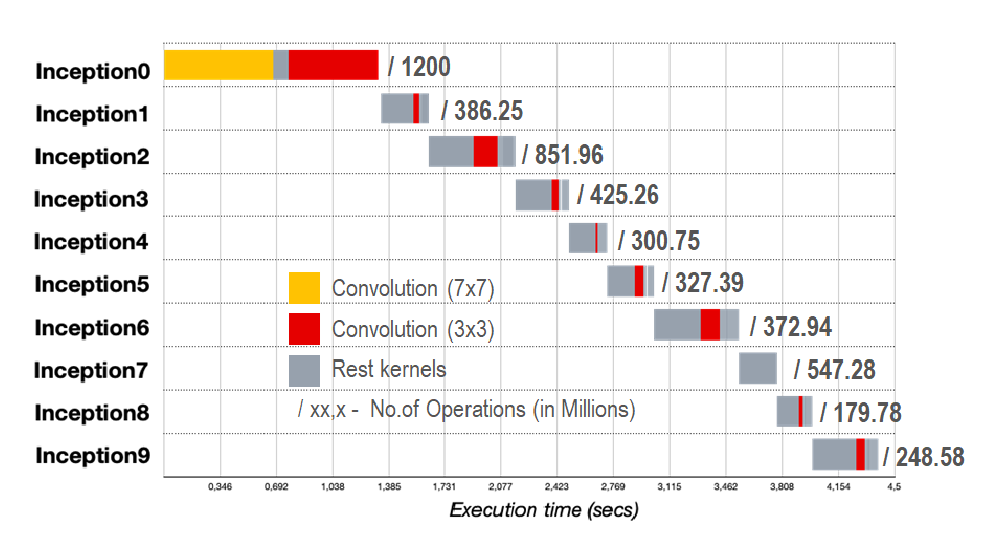
\includegraphics[width=\textwidth,height=\textheight,keepaspectratio]{img/GoogLeNetDSPOpt_Runtime_Graph.png}
  \caption{Execution time - GoogLeNet DSP Usage Optimized Design}
  \label{fig:GoogLeNetDSPOpt_Runtime_Graph}
\end{figure}


When the DSP usage optimized design was executed on all the 10 FPGAs, the design got executed in 4.41 seconds ! This was a noteworthy improvement in performance compared to the baseline design. 

The performance modeling for this design was not performed using the Antlr4 based tool. We were not able to extend the tool to account for the numerous changes that is present between the baseline design and the DSP usage optimized design.


\begin{table}[!htb]                          
 \centering
    \begin{tabular}{|c|c|}
    \multicolumn{2}{c}{\textbf{GoogLeNet DSP Usage Optimized : Performance Model}} \\ \hline

     No.of Operations    &   4.8 Billion \\ \hline
      Global Mem transfers &   20.9 GB            \\ \hline          
      Exe time    &  4410 ms    \\ \hline
      Operations/second   &   1.1 GOPS \\ \hline
      Operations/cycle &   8.66             \\ \hline
      Operations/byte       &   0.24 \\ \hline
      Global mem/second & 4.2 GBps  \\ \hline

    \end{tabular}
    \caption{GoogLeNet DSP Usage Optimized Performance Model}
    \label{tab:GoogLeNetDSPPerfModel}                            

\end{table} 

The performance modeling for the DSP usage optimized design is tabulated in Table \ref{tab:GoogLeNetDSPPerfModel}. Throughput, as defined in Chapter \ref{chp:Metrics}, for this design is 0.23 images classified per second. Since accuracy of the model is same as the one given in the literature (93.33\%), the only factor that could change when calculating Rate Correct Score is the latency. Similar to GoogLeNet baseline design, Rate Correct Score is calculated as the ratio between accuracy from literature and the latency of our implementation of GoogLeNet. For this design it is 21.16/s. 

We noticed two major problems from profiling data - stalling problem and memory dependency. In convolution kernels, the part where we were reading slices of data from global memory had stalls reaching 50\%. Since the  the part where the computations were taking place were directly dependent on these slices of data, the computations themselves had a disappointing occupancy of just 6.0\%. 

At this stage, we had the choice of thinking of ways to improve the design by sticking to the ongoing design paradigm or to think of a new approach. To show that further improvements could be done on the current design, we proceeded to implement extra optimizations on one single file. We picked a file (in this case inception9 file), completely unrolled the section of the code where slices of image-data were read, completely unrolled the section of the code where computations took place. When we synthesized this design and ran the resulting bitstream on the FPGAs (in conjunction with the previously used bitstreams), we saw a remarkable improvement in the run time of the convolution kernel on which we had applied the extra optimizations. Previously, this convolution kernel had taken about 79.06ms to get executed. But with the extra unrollings, this convolution kernel got executed in 1.75ms! The profiling data for this kernel execution showed that the resulting stall for the part of the code where slice of image-data was read was just 0.91\% and the part of the code where the computations were happening had an occupancy of 96.3\%.  

This proved that with some simple unrolls to the loops responsible for reading the slices of image-data and to the loops where computations were being done, we could achieve significant amounts of performance gain. As they say, there are no free lunches in the world of FPGA accelerators. All these unrolling demands resources and we were already running out of resources.


Even though the run time for DSP usage optimized design is about 15 times faster than the baseline version of GoogLeNet, there is a lot of room for improvement. Because of the problems related to synthesis of heavily unrolled designs discussed in the beginning of this subsection , we could not bank upon further unrolling of inner loops to gain performance improvements. Thus, we had to look elsewhere to improve the performance of our design.


This search for a better way to run GoogLeNet on multiple FPGAs resulted in our next design - GoogLeNet Hybrid Design.

\subsection{GoogLeNet Hybrid Design}
Designs which rely on global memory for data transfers tend to be slower than designs which make use of channels to transfer data from one kernel to another. This can be ascribed to the fact that global memory data transfers are slower than data transfers made using channels.  

Designs which are completely based on global memory data transfers need the host to take care of data transfers. When the amount of data to be transferred is large, this ends up being a significant overhead. Another problem with designs based on global memory is that the kernels have to be launched sequentially. Otherwise, the kernels end up working on garbage data. The host code is responsible for launching the kernels at the right time and to control the access to global memory. Because of sequential launching of kernels, a designer cannot exploit concurrent sections of a design in a straightforward manner. 

Considering the above points, we decided to implement GoogLeNet using channels. There are two types of channels available in Intel FPGA SDK for OpenCL - internal and external.

Internal channels are used to transfer data between kernels present in the same device. External channels, in our case, are direct point-to-point connections between two devices that are abstracted in the OpenCL environment as Serial Channels. There are four such IO channels per device. In terms of networking terminology these can be called : north, east, west and south channels. External channels make it possible to send data from kernels present in one device to kernels present in another device. 

To implement a channel-based design, we replaced all the data transfers within a kernel file with internal channels. We used blocking channels in our design. The inclusion of channels made it necessary to change the plug-in code (host code) to handle the launching sequence of the kernels. The plug-in was modified to launch all the kernels on separate command queues. This change allowed us to launch all the kernels in a kernel file simultaneously. 


\begin{figure}[!htb]
  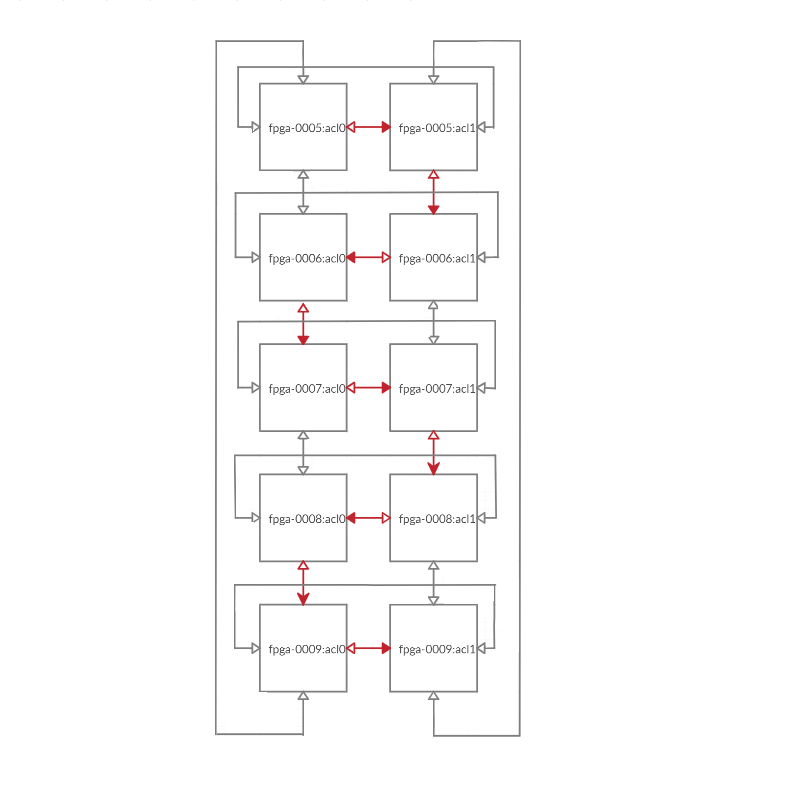
\includegraphics{img/Torus_Topology.PNG}
  \caption{Torus Topology}
  \label{fig:Torus_Topology}
\end{figure}

When it came to external channels, we had to choose between two designs : static design or dynamic design. With static design, the last kernel in a device is coded to output to a specific output channel and  the first kernel of a device is coded to read from a specific IO channel. This design would work great if the underlying hardware connections between different devices remain constant. If the point-to-point connections between two devices change for some reason, then one would have to rewrite the kernels to account for the change in topology, test them on emulators, put them for synthesis (which could take anywhere between 6 to 24 hours) and then try to run the new design on the new topology.




With dynamic design, instead of the first(last) kernel of a file reading(writing) from(to) one specific input(output) channel, the kernels could selectively read(write)  from(to) any one of the four IO channels available. By passing a "routing" argument and using if-else conditions in the first and last kernels of a file, it is possible to control the IO channels which feed-in or feed-out of a device. With dynamic design, it is possible to take routing decisions in the host code. Dynamic design helps in decoupling kernels from the underlying node topology.



If the routing decision is made in the host code, the routing decisions are made at compile time. This means that every time the node topology changes, one would have to change the routing parameters in the plug-in file, compile the plug-in and then run the design. We wanted to have routing decisions made at run-time to avoid this extra step of compilation. To this end, we outsourced the routing decision to a configuration file. We made use of an XML file where the node topology was described. This XML file was parsed during run-time to control the read/write operations on different IO channels. 

\begin{code}[!htb]
 \begin{minted}{XML}
<googlenet>
	<inception>
		<module>3a</module>           
		<input>0</input>				
		<output>3</output>
	</inception>
	<inception>
		<module>3b</module>
		<input>2</input>				
		<output>1</output>
	</inception>
...
...
...
	<inception>
		<module>5c</module>
		<input>2</input>				
		<output>0</output>
	</inception>
</googlenet>


\end{minted}
\captionof{listing}{Snippet of topology.xml}
\label{code:topologyxml}
\end{code}
Thus, dynamic design allowed us to write kernels which were independent of the underlying node topology. Since we had ten different files which were to run on ten different devices, we had to look for topology with ten devices. Such a topology was set up for us by the admin of Noctua Cluster. The resulting topology is shown in Figure \ref{fig:Torus_Topology}. The XML used for setting up the required connection is shown in Listing \ref{code:topologyxml}. The XML contains information about the CNN topology and the input channel and output channel for every inception file. The directions of the IO channels are enumerated as : 0- North, 1- South , 2- West, 3- East. For example, module 3b, which corresponds to inception1.aocx , needs the input to be read from channel 2 i.e. from channel arriving from the West and it needs to write data into channel 1 i.e. to the channel going to South.  
The filled red arrows in Figure \ref{fig:Torus_Topology} depict the routing paths we chose to scale over multiple devices. The grayed out connections were not used. We passed this XML file as an argument to our plug-in and parsed the information in the XML to get the final routing data. 

The introduction of internal and external channels in our design can be visualized from Figure \ref{fig:GoogLeNet_Channels}. The yellow arrows depict the external (IO) channels. The blue lines indicate the internal channels. Every inception module has 4 branches - branch0, branch1 , branch2 and branch3 - shown in Figure \ref{fig:GoogLeNet_Channels} as the branches going from left to right. The kernels in these branches can be launched concurrently with respect to kernels in other branches.  This was not possible in the earlier designs as we were using only one command queue to launch our kernels.

\begin{figure}[!htb]
  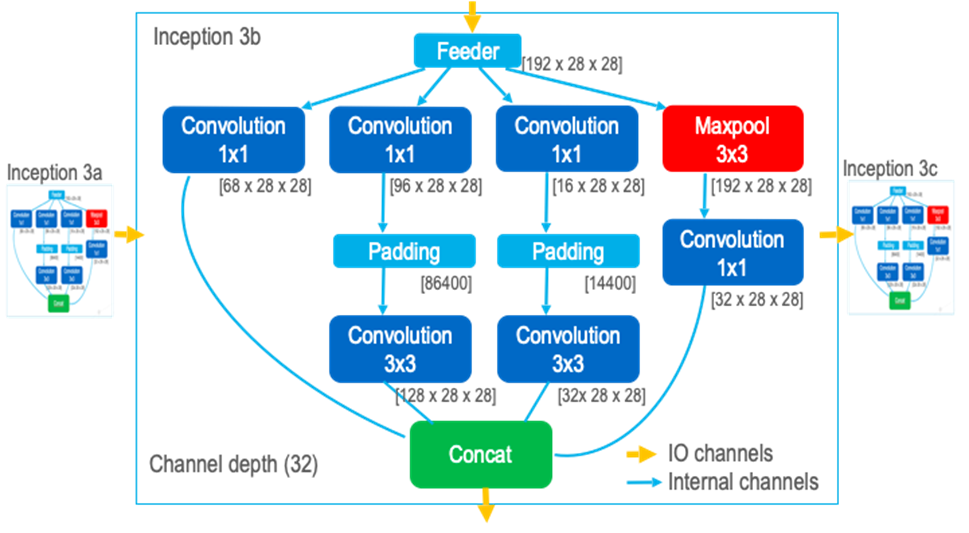
\includegraphics[width=\textwidth,height=\textheight,keepaspectratio]{img/GoogLeNet_Channels.png}
  \caption{GoogLeNet with Channels}
  \label{fig:GoogLeNet_Channels}
\end{figure}


Once all the files were converted to comply with channel-based design paradigm, we made the necessary modifications to the plug-in code. Before going for synthesis of the files, we made sure to test all the files on emulator. When the emulation was successful, we went ahead with synthesizing all the files into bitstreams.

When the bitstreams became available, we tried to run this new design on ten FPGAs. But to our dismay, this design just could not finish running on the FPGAs. It was stalling.

To find out why the design was not getting executed to completion, we went back to the kernel files, inserted "printf" statements to see the point until which the design was running successfully. When we did this, we found out that the design was stalling at the kernels which were feeding data to the Concatenation Kernel in inception1(3b) file. Since the team was working against time to get a fast design, we took a pragmatic approach towards solving this problem.

We replaced all the internal channels between Concatenation kernels (or Concat kernels) and the kernels feeding data to Concat kernels with global memory transfers. Since now we were making use of internal channels, external channels as well as global memory for transferring data, we decided to call this design as GoogLeNet Hybrid Design. Figure \ref{fig:GoogLeNet_Hybrid} depicts the hybrid design. 

\begin{figure}[!htb]
  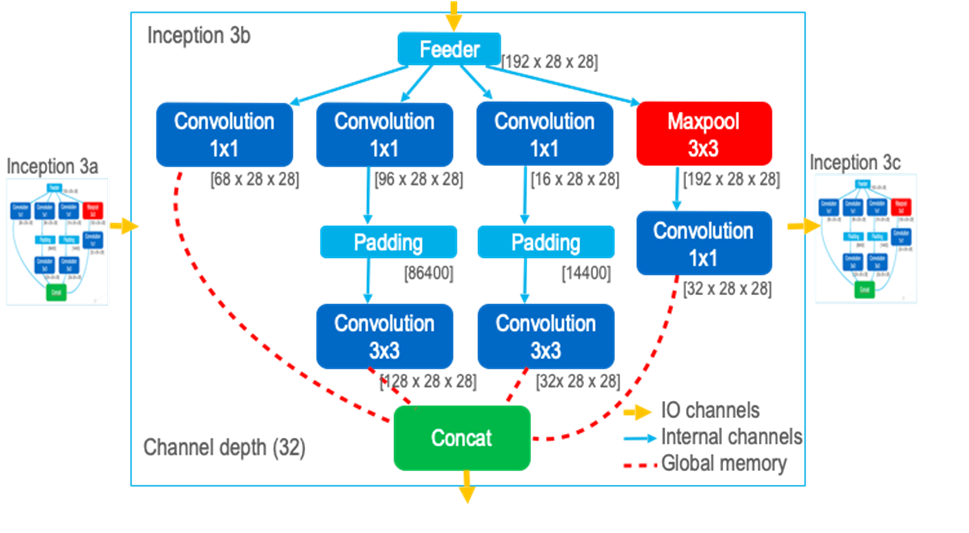
\includegraphics[width=\textwidth,height=\textheight,keepaspectratio]{img/GoogLeNet_Hybrid.PNG}
  \caption{GoogLeNet Hybrid Design}
  \label{fig:GoogLeNet_Hybrid}
\end{figure}

 Figure \ref{fig:GoogLeNet_Hybrid} shows how the internal channels between kernels of the 4 branches and Concat kernel was replaced with global memory. By doing this, we were able to get rid of the stalling problem which we faced in the "pure channels" version of the design.
 
 The global memory access between Concat and the kernels feeding to it required us to modify our plug-in code to launch Concat kernel in one of the four command queues of its feeders. We chose to launch Concat kernels on the same command queue as the 3x3 convolution of branch1. We had to call "clFinish()" for the command queues on which the terminal kernels of each branches were being launched before launching Concat kernel. This way we ensured that the Concat kernel worked on valid data from all the four branches.
 
 Having removed the stalling problem, we trained our sights on executing this design on ten FPGAs. This version of the design took 1.85 seconds to get executed ! The run time of this design is shown graphically in Figure \ref{fig:GoogLeNetHybrid_Runtime_Graph}.
 
 \begin{figure}[!htb]
  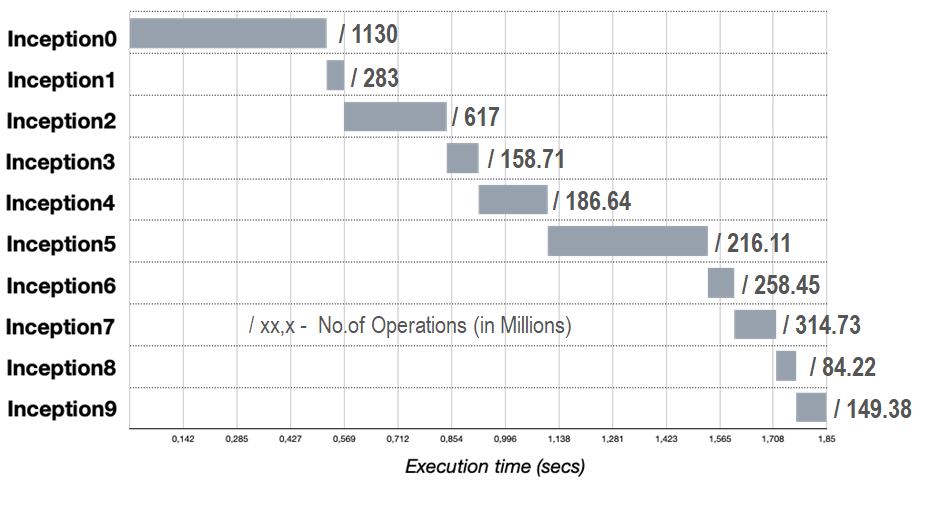
\includegraphics[width=\textwidth,height=\textheight,keepaspectratio]{img/GoogLeNetHybrid_Runtime_Graph.png}
  \caption{Execution time - GoogLeNet Hybrid Design Version 1}
  \label{fig:GoogLeNetHybrid_Runtime_Graph}
\end{figure}

Figure \ref{fig:GoogLeNetHybrid_Runtime_Graph} also indicates that the number of operations in this design in every kernel file is between the number of operations in baseline and DSP usage optimized designs. This is because a lot more optimizations were applied in DSP usage optimized design when compared to hybrid design. In terms of optimizations applied, hybrid falls in between DSP usage optimized and baseline designs.

By analyzing the profile.mon files, we realised that the design could have run faster if not for the bottleneck kernel files of inception0, inception2 and inception5.

To make this design faster, we decided to optimize inception0, inception2 and inception5 files. We referred to the profiling data of these kernel files to find out the bottlenecks within these files. For example, when we analysed the profile.mon of inception2 (3c module), we observed that the slowest branch (out of the 4 branches) was causing that part of the design run slowly. This can be observed from Figure  \ref{fig:GoogLeNet_Hybrid_Before_Opt}. 

 \begin{figure}[!htb]
  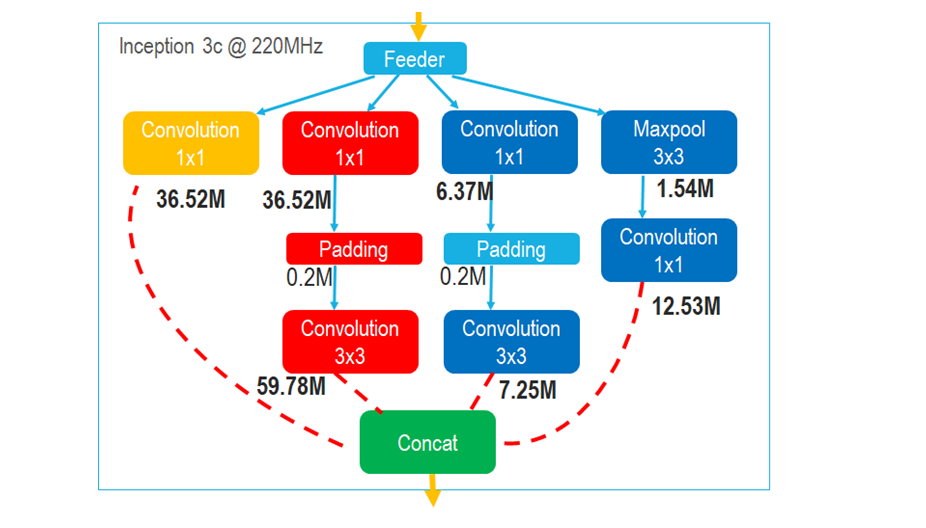
\includegraphics[width=\textwidth,height=\textheight,keepaspectratio]{img/GoogLeNet_Hybrid_Before_Opt.PNG}
  \caption{Number of clock cycles taken by kernels of different branches in inception2(3c) before resource redistribution}
  \label{fig:GoogLeNet_Hybrid_Before_Opt}
\end{figure}


As can be seen from Figure  \ref{fig:GoogLeNet_Hybrid_Before_Opt}, branch1,highlighted in red, requires about 96.5 million clock cycles to get executed - about three times slower than the next slowest branch.  With this design, this part of the design operated at a clock frequency of 220MHz.

We decided to make the kernels in branch1 faster by allocating more resources to it. The resources needed to make branch1 faster had to be taken away from the solitary kernel in branch0 for two reasons : 
\begin{itemize}
    \item the kernel in branch0 was under-performing. Even with a significant amount of resources allocated to it, it was performing relatively slow. In other words, the measured number of operation per cycle was less than the estimated number of operations.
    \item it is the only kernel in its branch. Rearranging the resources in branch2 and branch3 could have complex side effects.
\end{itemize}

When the resources were redistributed to make branch1 run faster, we noticed that the design got synthesized to run at a higher clock frequency - 285MHz. Compared to the previous design, this was an improvement of 65MHz. When we executed this modified design on hardware, we noticed that the run time went down for this particular bitstream. The analysis of profiling data of this new kernel file revealed that we were indeed able to reduce the run time of branch1. This can be seen from Figure \ref{fig:GoogLeNet_Hybrid_After_Opt} where we have documented the number of cycles needed for all the branches to get executed after the redistribution of resources.  

 \begin{figure}[!htb]
  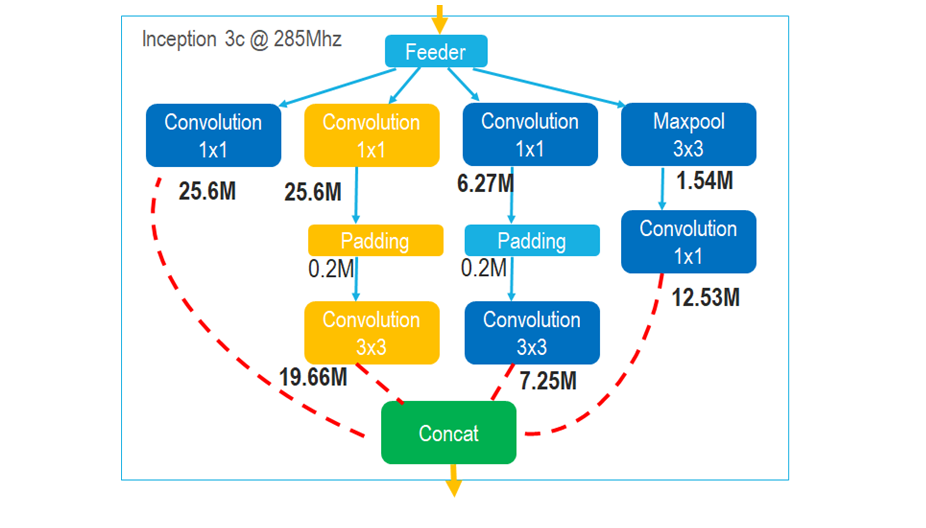
\includegraphics[width=\textwidth,height=\textheight,keepaspectratio]{img/GoogLeNet_Hybrid_After_Opt.png}
  \caption{Number of clock cycles taken by kernels of different branches in inception2(3c) after resource redistribution}
  \label{fig:GoogLeNet_Hybrid_After_Opt}
\end{figure}

The kernels of branch1 have been highlighted in yellow in Figure \ref{fig:GoogLeNet_Hybrid_After_Opt}. The number of clock cycles needed by branch1 to finish execution is about 45 million. This is twice as fast as the previous design. This reduction in required clock cycles and the increase in Fmax(clock frequency) meant the total run-time reduced by a fair margin.

We applied the same kind of optimizations on the other kernel files and the design took 1.18 seconds to classify one image. The relevant performance modeling parameters have benn tablulated in Table 


\begin{table}[!htb]                          
 \centering
    \begin{tabular}{|c|c|}
    \multicolumn{2}{c}{\textbf{GoogLeNet Hybrid Design : Performance Model}} \\ \hline

     No.of Operations    &   3.3 Billion \\ \hline
      Global Mem transfers &   1.9 GB            \\ \hline          
      Exe time    &  1180 ms    \\ \hline
      Operations/second   &   2.79 GOPS \\ \hline
      Operations/cycle &   12.15             \\ \hline
      Operations/byte       &   1.74 \\ \hline
      Global mem/second & 1.6 GBps  \\ \hline

    \end{tabular}
    \caption{GoogLeNet Hybrid Design Performance Model}
    \label{tab:GoogLeNetHybridPerfModel}                            

\end{table} 


Throughput, as defined in Chapter \ref{chp:Metrics}, for this design is 0.84 images classified per second. Since accuracy of the model is same as the one given in the literature (93.33\%), the only factor that could change when calculating Rate Correct Score is the latency. Similar to the other design design, Rate Correct Score is calculated as the ratio between accuracy from literature and the latency of our implementation of GoogLeNet. For this design it is 79.09/s.

In conclusion, we were able to create and execute different versions of GoogLeNet over multiple devices. We strongly believe we could have made our designs much better in terms of latency and throughput. During the last phase of the project, we were able to map out some future tasks to make our designs faster. These insights are discussed in section \todo{Link to future works}





 
 
 
 
 
 
 
 
 




























\section{ResNet-50}
The next CNN model we implemented was ResNet-50. While there are more deeper versions of ResNet present the sheer workload of executing them was too much. ResNet-50 was deep enough to achieve the objective of scaling as stated in the project goals. During the implementation of GoogleNet we came across some unforeseen roadblocks which took time to be resolved. However, the team was quick to rectify the mistakes from the lessons learned during previous implementation. This enabled the team to execute several versions of ResNet-50 ranging from the baseline architecture to a more optimised and faster version of the model at a faster pace than before.
We were able to implement four versions for ResNet-50:
\begin{itemize}
    \item ResNet Baseline
    \item ResNet Opt-V1
    \item ResNet Opt-V2
    \item ResNet Opt-V3
\end{itemize}

\subsection{ResNet Baseline}
The method to implement ResNet-50 was very similar to that of GoogleNet baseline architecture. We first generated all the kernel files that were needed to execute the ResNet-50 architecture. After the generation of the kernel files we observed that the number of kernels generated by TVM was less than what our OpenVINO IR was expecting. The reason for this is that in the ResNet-50 architecture there are many of the kernel files whose dimensions are exactly the same. So TVM does not generate the duplicate kernels and only generates the kernels which are not same. This behaviour was opposite to what we saw in GoogleNet where TVM generated more kernels than what was expected. This warranted some extra efforts apart from some pre-optimization tasks that were done to execute the baseline version.
Some of the mandatory modifications done were:
\begin{itemize}
    \item renaming kernel names to match with OpenVINO IR
    \item merging ReLUs with convolutions
    \item removing transpose kernels
    \item duplicating the required kernels not generated by TVM
\end{itemize}
 After the completion of these pre-execution steps the modified code was complied to run on FPGA emulator for Intel Stratix 10 using the latest toolchain-19 of the Board Support Package. Again the functional correctness was checked by comparing the output of our design with the output from TensorFlow implementation. Our modified ResNet-50 code was functionally correct and gave us the right score and label for the image we fed to it. The next obvious step for us then was to implement this baseline version on actual Intel Stratix 10 FPGAs.
 \newline
 In doing so we first looked into the initial report of the entire ResNet-50 architecture which was just a single file. The report, as shown in Figure \ref{fig:ResNet50_baseline_report}, indicated that it is impossible to execute the baseline version on just a single FPGA since our design surpassed the available resources present on the board. This was expected and warranted us to divide the entire architecture into smaller executable parts.
 
 \begin{figure}[!htb]
  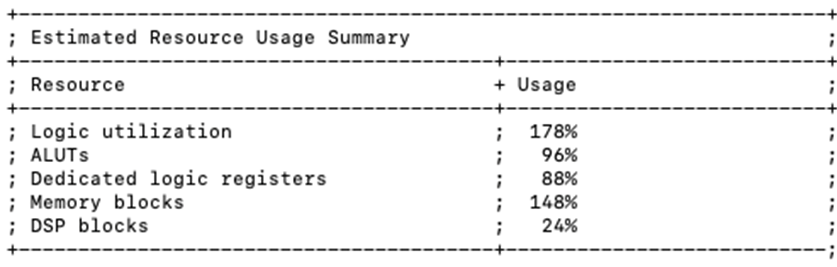
\includegraphics[width=\textwidth,height=\textheight,keepaspectratio]{img/ResNet_baseline.png}
  \caption{Resource Summary - ResNet-50 Baseline Architecture}
  \label{fig:ResNet50_baseline_report}
\end{figure}

We made use of inherent logical divisions present in the ResNet-50 architecture in form of blocks. The entire topology was divided into 5 blocks namely from block1 - block4 with 4 block consisting of 3 units and 1 block consisting of 4 units. The end of each unit was marked by a eltwise kernel which was used as a separation criterion. So at the end of every $3^{rd}$ unit for block1, block3\_1, block3\_2 and block4 a block was formed and block2 was formed at the end of its $4^{th}$ unit. We planned on scaling it to 5 FPGAs with each FPGA being allocated to a  single block. 
After the division of the entire topology into 5 blocks we did not exceed resource utilization requirement and were able to generate the bitstreams and execute it on FPGAs. Since the flashing logic was developed during GoogleNet implementation phase, we adopted the same logic and code with changes in the parity calculations as we were flashing only 5 bitstreams and not 10.   

Global memory was used for intra-node communication and MPI was used to transfer data from one node to another. Here the MPI\_Send() was called at the last of block2 and block3\_2 eltwise kernel except for the last block. MPI\_Recv() was called at the beginning of block3\_1 and and block4.

\begin{figure}[!htb]
  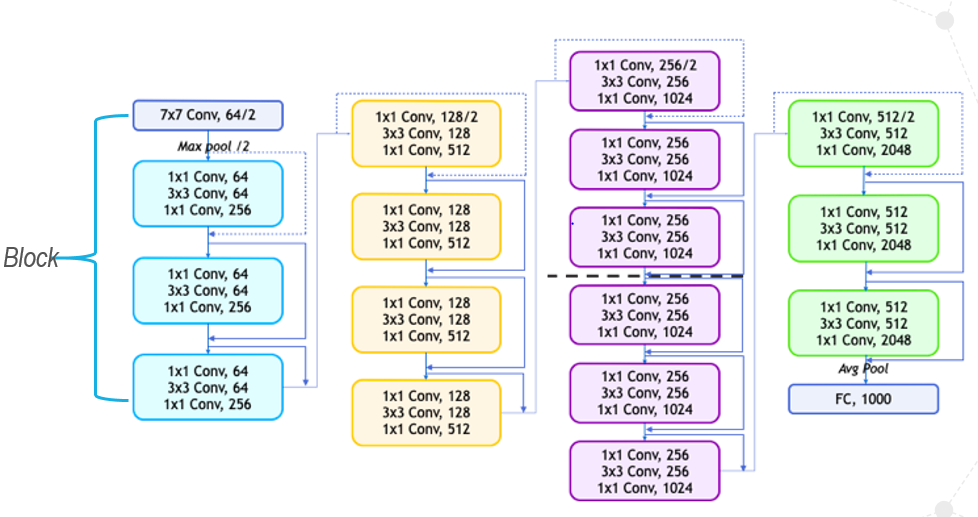
\includegraphics[width=\textwidth,height=\textheight,keepaspectratio]{img/ResNet_division.png}
  \caption{Division of ResNet-50 Baseline Architecture}
  \label{fig:ResNet50_baseline_division}
\end{figure}


One thing to note here is that the baseline version does not contain any kind of optimizations. Practically it is a good practice to pipeline all the loops and bring all II to 1, we chose to execute this out-of-the-box design to gain insights on its performance measure.
As expected the baseline was slow and took 117.34 seconds to classify a single image. The run-time performance of this design can be visualized from Figure \ref{fig:ResNet50_baseline_time}. This is a very slow design and needs to be optimised. However, this design served as a reference point for future comparison on the performance gains which will be achieved with optimised designs.

\begin{figure}[!htb]
  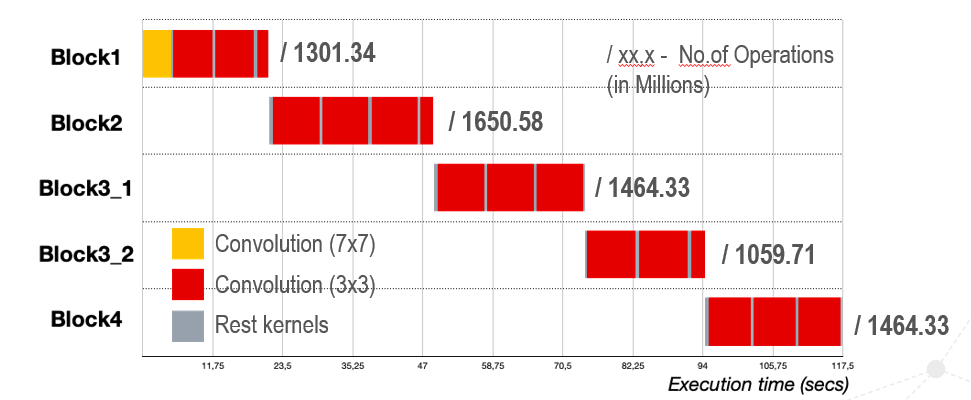
\includegraphics[width=\textwidth,height=\textheight,keepaspectratio]{img/ResNet_baseline_execution.png}
  \caption{Execution time - ResNet-50 Baseline Architecture}
  \label{fig:ResNet50_baseline_time}
\end{figure}


\begin{table}[]
\centering
\captionsetup{
justification = centering
}
\caption{ResNet-50 Baseline Performance Model}
\label{tab:ResNetBaselinePerformanceModel}
\begin{tabular}{|c|c|}
\hline
Number of Operations     & 6.94 Billion \\ \hline
Global Memory transfers & 65.90 GB     \\ \hline
Execution time             & 117345 ms    \\ \hline
Operations/second    & 0.23 GOPS    \\ \hline
Operations/cycle     & 0.29         \\ \hline
Operations/byte      & 0.09         \\ \hline
Global Memory/second    & 576 MBps     \\ \hline
\end{tabular}
\end{table}

We learned that most of the execution time was being spent in 3x3 convolution kernels. Optimising these kernels was a priority. Also due to large II and loop carried dependencies the number of clock cycles needed to execute these kernels was very high. Another factor that contributed to the slow execution was the under-usage of DSP blocks. Less than 1\% of DSP blocks were being used. Since it is the baseline version, no loop unrolling was implemented which could effectively increase the number of MAC operations executing in a single cycle. Due to this at most two MAC operations would be executed in theory. However, looking into the profiling data provided by the respective profile.mon files of each block we observed that our kernels had very less occupancy on FPGAs for raw kernel execution and low read/write efficiency from global memory. The suspected reason for such low efficiency was random global memory accesses by our kernels. So optimising our memory access pattern was also a crucial step in moving forward. Because of all of these factors the measured value which was 0.16 ops/cycle was way less than the 2 ops/cycle estimate. The performance model for this design has been tabulated in Table \ref{tab:ResNetBaselinePerformanceModel}.  
Throughput, as defined in Chapter \ref{chp:Metrics}, for this design is 0.008 images classified per second. Since  the Top-5 accuracy of the model is the same as the one given in the literature (93.29\%), the only factor that could change when calculating Rate Correct Score is the latency. And for this case , Rate Correct Score is calculated as the ratio between accuracy from literature and the latency of our implementation of ResNet-50. This comes to be  0.79 per second.
\newline
Reasons for poor performance of baseline version are:
\begin{itemize}
    \item II greater than 1 
    \item No loop pipelining
    \item Inefficient global memory access patterns
    \item Low DSP usage
    \item Due to serial architecture FPGAs are idle most of the time
\end{itemize}
To summarize the baseline version was very slow and needed to be optimised.

\subsection{ResNet Opt-V1}
The performance of the baseline version was not acceptable and in real world scenarios the latency time was too high to be used. Therefore, there was a need to optimise the baseline version. As mentioned in the previous section the baseline version was completely devoid of any kind of optimization and the major bottleneck was the 3x3 convolution kernel which were responsible for high execution time. Also from the profile.mon file of the kernels from the baseline version as seen in Figure \ref{fig:ResNet50_baseline} the team learned that kernels had very less occupancy on FPGA and also the read/write efficiency was also very less. Optimising and increasing the efficiency and occupancy was one of the main objectives of this optimization phase. The optimization queue had the following tasks:
\begin{itemize}
    \item Loop pipelining
    \item Loop unrolling
    \item Using local memory 
    \item Use of temporary variables
\end{itemize}

\begin{figure}[!htb]
 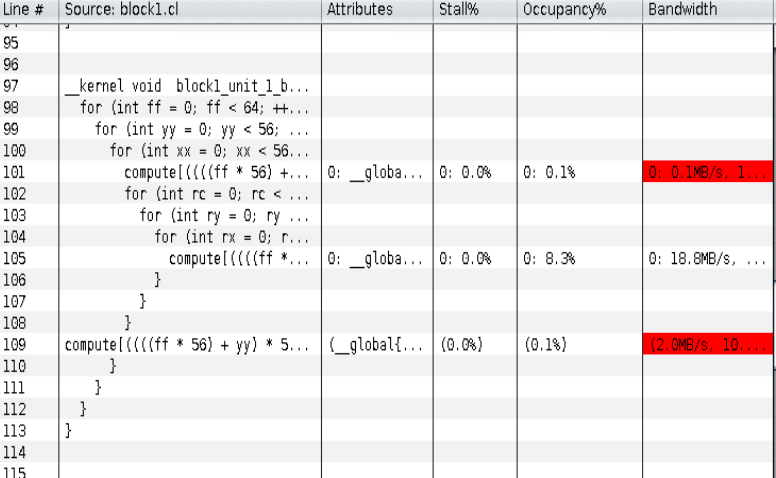
\includegraphics[width=\textwidth,height=\textheight,keepaspectratio]{img/Baselinebottleneck.png}
 \caption{ResNet Baseline Bottleneck Analysis}
 \label{fig:ResNet50_baseline}
\end{figure}

The block-wise divided design was taken to carry out the above mentioned optimizations. All the weights and biases were stored in local memory. Since the sizes of weights and biases were small, storing them in local memory was feasible. This reduced the effort to read everything from the global memory thereby helping in reducing the overall read/write time. Also with the introduction of temporary variables to store the intermediate results getting rid of loop carried dependencies became easy. Furthermore, wherever possible loop unrolling was carried out to increase instruction level parallelism. All of these optimizations resulted in a kernel design in which all the loops were pipelined and it was possible to execute multiple operations in every clock cycle.
\newline
The resource utilization after carrying out these optimizations as seen in Figure \ref{fig:ResNet50_optv1_usage} was under the allowed capacity. One thing to observe is that even though the utilization of the memory blocks increased significantly it is not a true measure of performance metric. Also the DSP utilization is about 2\% which is less and needs to increased. However, it was to be seen how the kernels performed after these set of optimizations and therefore increasing DSP utilization was given low priority at this stage.

\begin{figure}[!htb]
 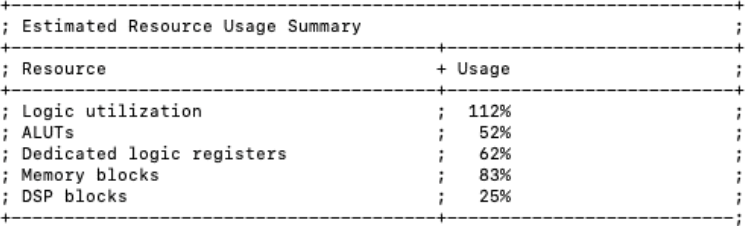
\includegraphics[width=\textwidth,height=\textheight,keepaspectratio]{img/resnetv1ru.png}
 \caption{Resource Summary - ResNet-50 Opt-V1 Architecture}
 \label{fig:ResNet50_optv1_usage}
\end{figure}

After successful functionality testing, bitstreams for all the kernel files were generated and the design was executed on 5 FPGAs. There was a significant increase in performance gain and the entire topology executed in 10.77 seconds. The performance gain was 10$\times$ as compared to the baseline version. This increase in speed was significant and goes to show how loop pipelining and unrolling can have significant impact on performance of a kernel.
\newline
Now the profiling data of these kernel files were analysed. After closer observation of the profile.mon data, we noticed that the occupancy and efficiency parameters, which were crucial in deciding the run-time, had improved. The kernels had high occupancy i.e they spend more time on computation and also the clock frequency of these kernels improved from the previous version. The graph in Figure \ref{fig:ResNet50_optv1_execution} gives the division of the entire run-time. In the baseline version, the run-time for Block1 was around 23 seconds whereas in ResNet Opt-V1, run-time for Block 1 was around 2 seconds. In similar manner all other blocks showed speed-ups in execution time. The entire performance model for this design is tabulated in Table \ref{tab:ResNet50OptV1PerformanceModel}.  

\begin{table}[!htb]
\centering
\captionsetup{
justification = centering
}
\caption{ResNet-50 Opt-V1 Performance Model}
\label{tab:ResNet50OptV1PerformanceModel}
\begin{tabular}{|c|c|}
\hline
Number of Operations     & 7.6 Billion \\ \hline
Global Memory transfers & 13.29 GB    \\ \hline
Execution time             & 10777 ms    \\ \hline
Operations/second    & 6.57 GOPS   \\ \hline
Operations/cycle     & 37.73       \\ \hline
Operations/byte      & 5.32        \\ \hline
Global Memory/second    & 1.234 GBps  \\ \hline
\end{tabular}
\end{table}


Throughput, as defined in Chapter \ref{chp:Metrics}, for this design is 0.09 images classified per second. Since  the Top-5 accuracy of the model is the same as the one given in the literature (93.29\%), the only factor that could change when calculating Rate Correct Score is the latency. And for this case , Rate Correct Score is calculated as the ratio between accuracy from literature and the latency of our implementation of ResNet-50. This comes to be  8.66 per second.  


In this version, as we can see from the graph shown in Figure \ref{fig:ResNet50_optv1_execution}, the bottleneck were 1x1 convolution kernels as opposed to 3x3 convolution kernels in the baseline version. The occupancy of these 3x3 kernels was around 99\% with better clock frequency. These set of optimizations solved the major problem which was prevalent in the baseline version. 

\begin{figure}[!htb]
 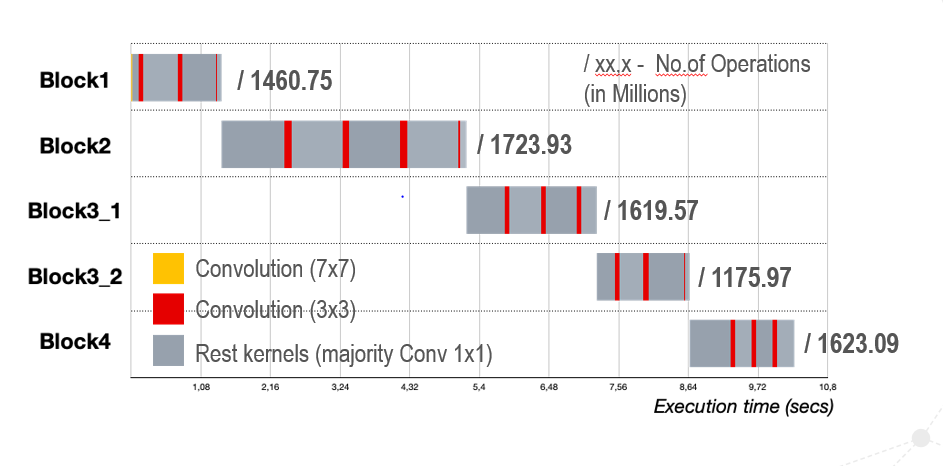
\includegraphics[width=\textwidth,height=\textheight,keepaspectratio]{img/resnetv1exe.PNG}
 \caption{Execution Time - ResNet Optv1 }
 \label{fig:ResNet50_optv1_execution}
\end{figure}

As mentioned earlier DSP blocks were under utilized and increasing it was an imperative step. This warranted a completely different design than what was being executed till now. This resulted in the next version namely ResNet Opt-V2 which will be discussed in the following section.



\subsection{ResNet Opt-V2}
The optimizations performed on the baseline architecture proved to be very effective and provided great result. The performance gain was 10$\times$ from the baseline version. Despite having a promising result there was an opportunity to optimise it further and get a better result. The main reason to go forward with another iteration of optimisation was due to low utilization of the available resources on the board, especially the DSP blocks. Even with the Opt-V1 version the amount of DSP blocks that were used was at most 2\% and the rest was used by the BSP. The main objective of this iteration was to increase the DSP utilization by a significant percentage as an increase in DSP will result in execution of more operations in a single clock cycle. In the previous version of ResNet-50 at most 84 operations per cycle or on an average 15 operations per cycle were being executed due to partial unrolling.
\newline
Till now the topology was divided block-wise with each block containing certain number of units. However, there was a need to completely unroll the inner loops if more DSP blocks were to be used. The current division did not allow that to happen. Therefore, there was a need to divide the entire topology in a completely different way. The next step was to divide it unit wise since the units in itself were very small and allowed for further optimizations. The unit-wise division led to creation of 16 units which will be flashed on 16 FPGAs as opposed to 5 FPGAs from Opt-V1 version. This also led to changes in the Open VINO FPGA plugin since it had to be adapted to the new unit-wise division. The parity calculation for flashing the aocx needed to be modified. The team estimated that there will be significant increase in performance gain of the kernels by increasing the utilization of the DSP blocks and flashing on more FPGAs. 
\newline
The team adopted the strategy implemented during the GoogleNet DSP Usage Optimized phase. The idea was the same. All the operations were executed in the spatial dimension first and then one channel deeper. This happens till all the pixels are operated upon. At this stage the innermost loops were fully unrolled. This resulted in two things. One, the DSP utilization was increased to almost 50\% and second, FPGAs do not have to have to wait for the entire data to be read which would further decrease the kernel execution time. The weights and biases were also copied to local memory reducing global read/write accesses. It was estimated that more than 100 operations per cycle would get executed. 
\begin{figure}[!htb]
  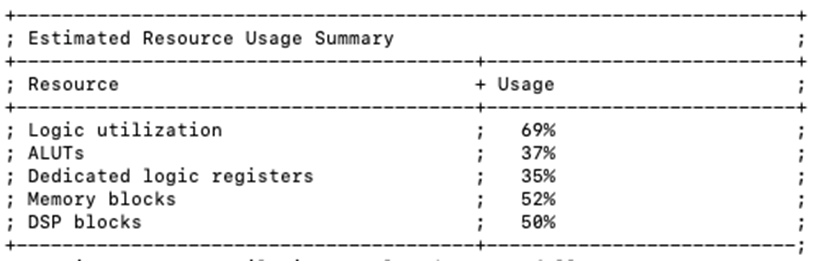
\includegraphics[width=\textwidth,height=\textheight,keepaspectratio]{img/ResNet_DSP_usage.png}
  \caption{Resource Summary - ResNet-50 Opt-V2 Architecture}
  \label{fig:ResNet50_Optv2_usage}
\end{figure}
\newline
When this design was sent for synthesis, as expected the synthesis failed either during the fitter placement or fitter routing phase. Just like GoogleNet we had to reduce the number of DSP blocks being used and send it again for synthesis. However, after reducing the DSP percentage once or twice the kernels were being synthesized. After generation of all the bitstreams the topology was executed on 16 FPGAs and the run-time was 16.49 seconds. Figure \ref{fig:ResNet50_Optv2} shows the run-time of all the 16 units.

\begin{figure}[!htb]
  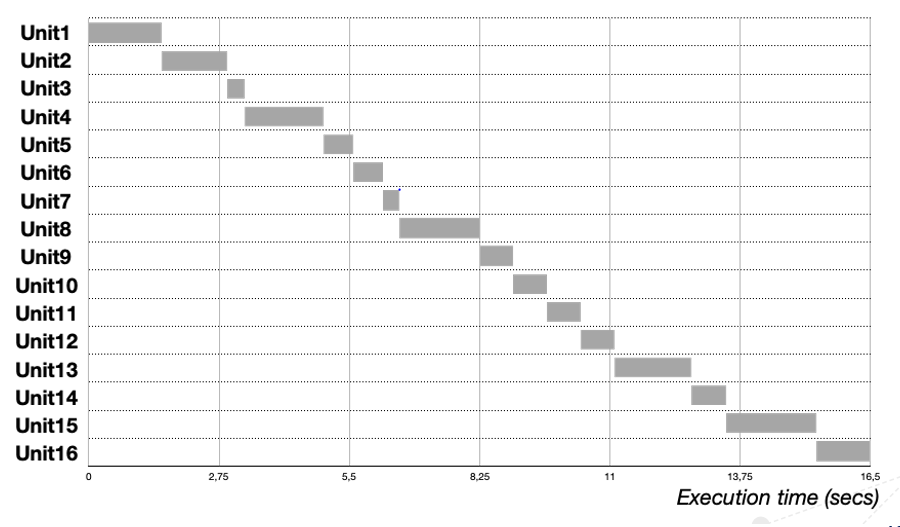
\includegraphics[width=\textwidth,height=\textheight,keepaspectratio]{img/ResNet_DSP.png}
  \caption{Execution time - ResNet-50 Opt-V2 Architecture}
  \label{fig:ResNet50_Optv2}
\end{figure}

According to the estimations the entire topology with this new design should have completed its execution in under 1 second. However, this was not the case and needed deeper investigation to find out the root cause of the problem. When the profiling data of these units were analysed it was found that even though the performance of some of the kernels got better, many of the kernels did not perform as expected. There were two reasons for that:
\begin{itemize}
    \item Stalling problem 
    \item Memory dependency
\end{itemize}
This problem was similar to what we had previously encountered with GoogleNet for the same optimised DSP design. Here the stalling percentage was more than 66\% and the occupancy for raw kernel execution was less on FPGA. At this stage the resource utilization was not high but due to synthesis problem there was no more room to optimize it further i.e perform more loop unrolling to block of code where the image slices are being read. Also the time to synthesize a single kernel file was more than 12 hours on average. This severely limited our opportunities for more optimizations. 
\newline
Due to the above mentioned reasons and the kernel computation logic scaling to 16 FPGAs did not perform the way it was expected to perform. Also due to the synthesis problems and time constraint to meet the project deadline the team could not afford to spend more time on this version of ResNet-50. There was a need to find a new way to optimise these kernels in a way that will increase the execution performance. Therefore, the team decided to execute one more version of ResNet-50 in hope to have better performance gain which resulted in ResNet Opt-V3.
\subsection{ResNet Opt-V3}
In ResNet Opt-V2 the performance of the overall topology was not optimal. There were stalling and memory dependency problems which needed to be resolved. The team needed time and resources to solve this. However, the team was bounded by two constraints: 
\begin{itemize}
    \item Project deadline 
    \item Unavailability of Noctua Infrastrcture due to maintanence 
\end{itemize}
By the time execution of ResNet Opt-V2 was finished the team had very less time of approximately 6-7 days to do any kind of modifications to the existing design and synthesize it again. To our dismay the date of the of the project deadline and maintenance of the Noctua infrastructure conincided which left us with less time to do any kind of optimisation. ResNet Opt-V2 had a runtime of 16.49 seconds whereas ResNet Opt-V1 had runtime of 10.77 seconds. Therefore, the team decided to optimize the ResNet Opt-V1 further as it had shown promising result till now. The idea of optimising it further was taken from the ResNet Opt-V2 i.e streching the design to 16 FPGAs. ResNet Opt-V3 was an amalgamation of the previous two optimization efforts. 
\newline
Here again the entire topology was divided into units instead of blocks. The computaton logic was same as that of the ResNet Opt-V1 i.e the operation takes place in depth dimension first and then spatially. Since this was a unit-wise division there was room to perform loop unrolling. The kernels were pipelined and no extra efforts was needed in that respect. In this version it was possible to fully unroll the innermost loops which were partially unrolled due to resource constraint in ResNet Opt-V1. Optimization priority was given to those kernels which had under performed in the ResNet Opt-V1 which were the 1x1 convolution kernels. 
\newline
Most of the complete loop unrolling took place in the 1x1 convolution kernels. However not every 1x1 convolution kernel was completely unrolled. Every unit consisted two of these slow 1x1 convolution kernels. At any given time only one of these two kernels could be completely unrolled at the beginning of the topology since the dimensions of the image were big. If both of these kernel were completely unrolled, it resulted in high resource utilization thereby rendering the kernel file incapable of being synthesized. As the network got deeper and dimensions of the image started getting small in some units it was possible to completely unroll both the 1x1 convolution kernels. While unrolling the innermost loops it was observed that the DSP utilization was also increasing. However, from past experience it was clear that high DSP utilization would result in synthesis failure. Therefore, it was decided to keep DSP utilization under 35\%. In such fashion all the 16 units were optimised, tested and sent for synthesis. 
\begin{table}[!htb]
\centering
\captionsetup{
justification = centering
}
\caption{ResNet-50 Opt-V1 Performance Model}
\label{tab:ResNet50OptV3PerformanceModel}
\begin{tabular}{|c|c|}
\hline
No.of Operations     & 6.96 Billion \\ \hline
Global Mem transfers & 52.18 GB     \\ \hline
Exe time             & 12105 ms     \\ \hline
Operations/second    & 0.535 GOPS   \\ \hline
Operations/cycle     & 2.63         \\ \hline
Operations/byte      & 0.12         \\ \hline
Global mem/second    & 4.31 GBps    \\ \hline
\end{tabular}
\end{table}
After modifying and testing the kernels from ResNet Opt-V1 team had only 4 days to synthesize 16 designs. The timeline was very tight as some of the kernels might take a long time to get synthesized. Four to five designs were put to synthesis in parallel to meet the maintenance deadline. During synthesis some of the designs failed to synthesize and had to be modified again i.e reduce unroll factors. Due to this by the end of the deadline 13 design got synthesized and synthesis of 3 designs namely unit 13, unit 14 and unit 15 was unsuccessful. 
\newline
To execute the entire topology 16 bitstreams were needed. The remaining 3 bitstreams was taken from ResNet Opt-V2. While executing this version of ResNet the plugin was not able to parse beyond the eltwise kernel of 4 units namely unit 3, unit 9, unit 10 and unit 12. The reason for that is till unknown as nothing was changed in those kernels. The bitstreams for those 4 units were taken from ResNet Opt-V2. In total there were 9 units from ResNet Opt-V3 and 7 units from ResNet Opt-V2 used to run the network. Therfore ResNet Opt-V3 was a mixture of two version of optimizaton. 
\newline
It was possible to run the network on FPGA. After successful execution of the network the runtime obtained was 12.105 seconds. This execution time was better than ResNet Opt-V2 but had degraded in comparison to ResNet Opt-V1. 
\begin{figure}[!htb]
  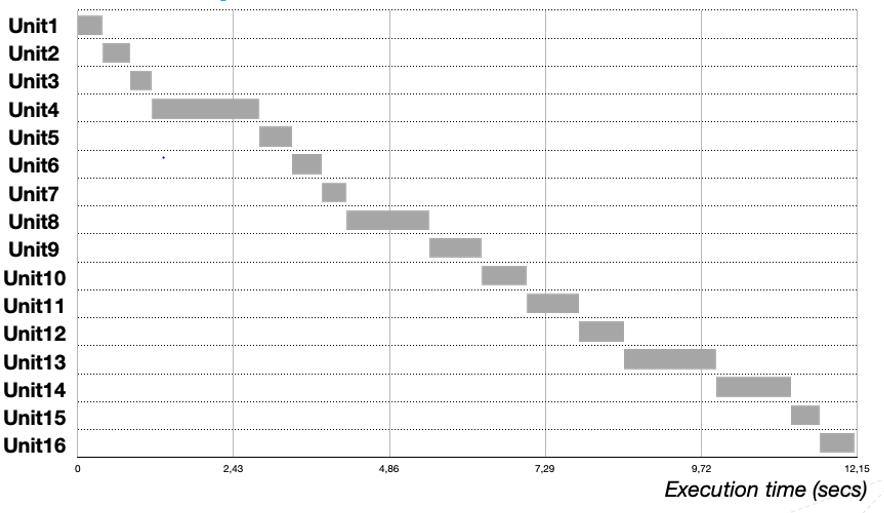
\includegraphics[width=\textwidth,height=\textheight,keepaspectratio]{img/ResNet_OptV3_execution.png}
  \caption{Execution time - ResNet-50 Opt-V3 Architecture}
  \label{fig:ResNet50_Optv3}
\end{figure}
Profiling data data showed that the performance of units from ResNet Opt-V3 had become better than their ResNet Opt-V1 counterpart. This can be illustrated in Fig \ref{fig:ResNet50_Optv3_kernel}. In this unit the block1\_unit1\_bt\_v2\_conv2\_Conv2D kernel executed in around 400 ms whereas the same kernel took 1.46 seconds to execute in ResNet Opt-V1. This was 3$\times$ performance gain. In similar manner kernels from other units of ResNet Opt-V3 design showed speed up. Due to the usage of 7 designs from the pervious ResNet Opt-V2 version the execution time increased as the unit themselves were slow from that version. 
\newline
The main takeaway from this version is that ResNet-50 could have been executed in less 10.77 seconds if only we had all the units completely optimised. However, the team was able to create and execute different versions of ResNet over multiple devices. We definetely could have done much better but the team faced some tough challenges during the entire development phase. These challenges will be discussed in \ref{sec:challenges}

\begin{figure}[H]
  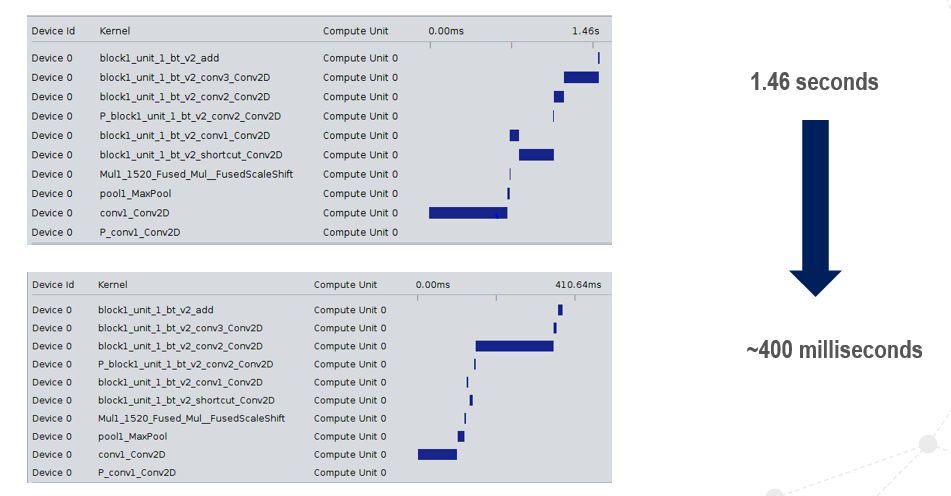
\includegraphics[width=\textwidth,height=\textheight,keepaspectratio]{img/ResNet_OptV3_performance.png}
  \caption{Execution time - ResNet-50 Opt-V3 Architecture}
  \label{fig:ResNet50_Optv3_kernel}
\end{figure}
%End of the chapter